\begin{center}
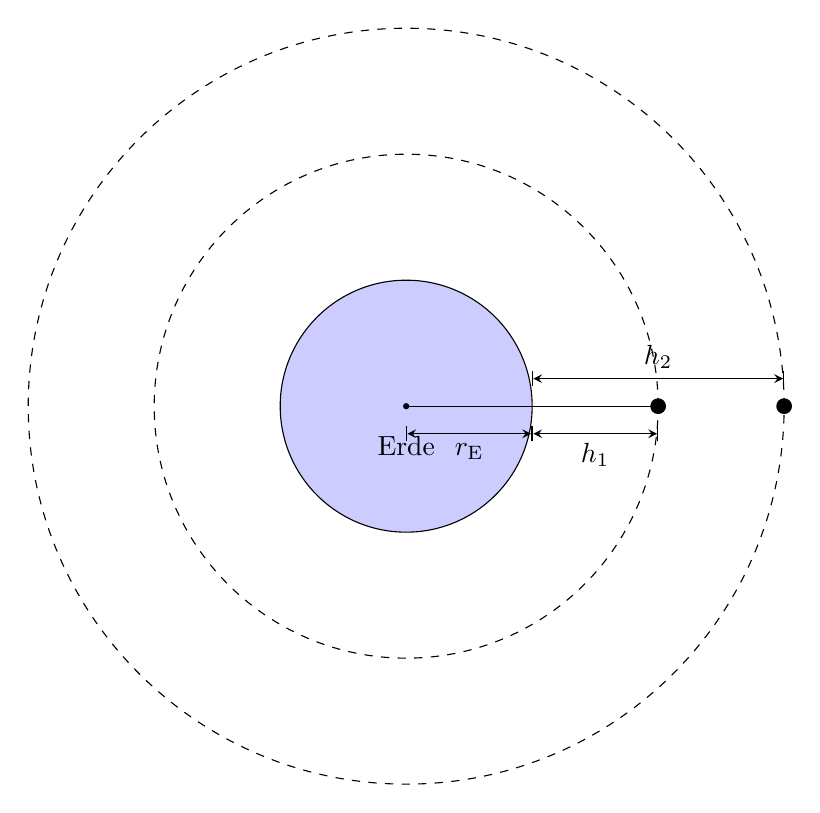
\begin{tikzpicture}[>=stealth]
 \fill[blue!20] (0,0) circle (1.6);
 \draw (0,0) circle (1.6);
 \fill (0,0) circle (0.04);
 \node at (0,-0.5) {Erde};

 \draw[dashed] (0,0) circle (3.2);
 \draw[dashed] (0,0) circle (4.8);
 \draw (0,0) -- (3.2,0);
 \fill (3.2,0) circle (0.1);
 \fill (4.8,0) circle (0.1);
 \draw[|<->|] (0,-0.35) -- (1.6,-0.35) node[midway, below] {$r_\mathrm{E}$};
 \draw[|<->|] (1.6,-0.35) -- (3.2,-0.35) node[midway, below] {$h_1$};
 \draw[|<->|] (1.6,0.35) -- (4.8,0.35) node[midway, above] {$h_2$};
\end{tikzpicture}
\end{center}

Die Gravitationsenergie hängt vom Abstand $r$ zum Erdmittelpunkt ab, nicht von der Höhe über der Oberfläche:
\begin{align}
 E_\mathrm{p} &= -G\,\frac{M_\mathrm{E}\,m}{r}
\end{align}
Bei der Flughöhe $h_1 = r_\mathrm{E}$ ist $r_1 = 2\,r_\mathrm{E}$, bei $h_2 = 2\,r_\mathrm{E}$ ist $r_2 = 3\,r_\mathrm{E}$. Damit
\begin{align}
 \frac{E_\mathrm{p,2}}{E_\mathrm{p,1}} &= \frac{r_1}{r_2} = \frac{2\,r_\mathrm{E}}{3\,r_\mathrm{E}} = \result{\frac{2}{3}}
\end{align}
Die (negative) Gravitationsenergie wird betragsmässig um den Faktor $\frac{2}{3}$ kleiner, d.\,h. sie nimmt zu.
